%! Author = gra
%! Date = 23.03.24

% Preamble
\begin{flushleft}
    \paragraph{yugabyteDB}
    Zuerst wurde für die Annährend 5GiB-DB initialisiert:
\lstset{style=gra_codestyle}
\begin{lstlisting}[language=sql, caption=yugabyteDB - Benchmarking - DB erstellen,captionpos=b,label={lst:yugabytedb-benchmarking-create-db},breaklines=true]
yugabyte=# create database pgbench_eval_bench;
CREATE DATABASE
\end{lstlisting}


    \subsubsection{Benchmarks}
    Die Auswertung anhand der tps
    \begin{figure}[H]
        \centering
        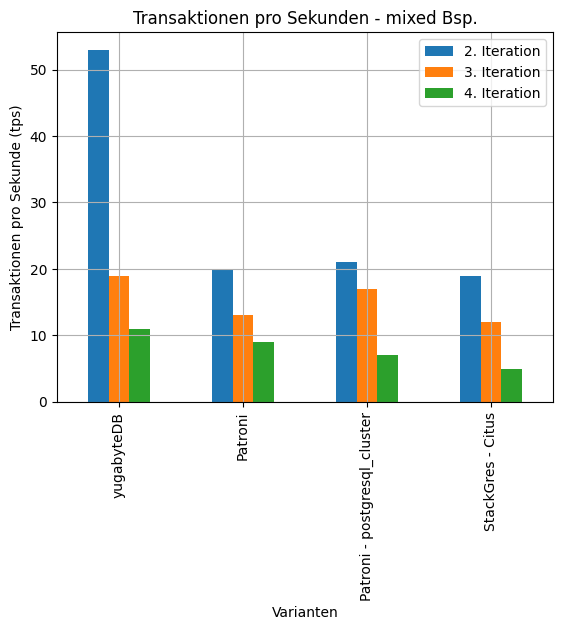
\includegraphics[width=1\linewidth]{source/pandas_data_chart_plotter/tps_mixed}
        \caption{Benchmarks - tps mixed}
        \label{fig:tps_mixed}
    \end{figure}

    \begin{figure}[H]
        \centering
        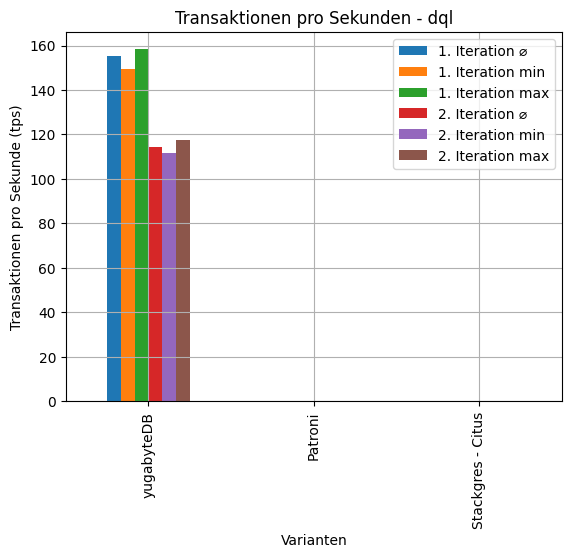
\includegraphics[width=1\linewidth]{source/pandas_data_chart_plotter/tps_dql}
        \caption{Benchmarks - tps dql}
        \label{fig:tps_dql}
    \end{figure}

    \begin{figure}[H]
        \centering
        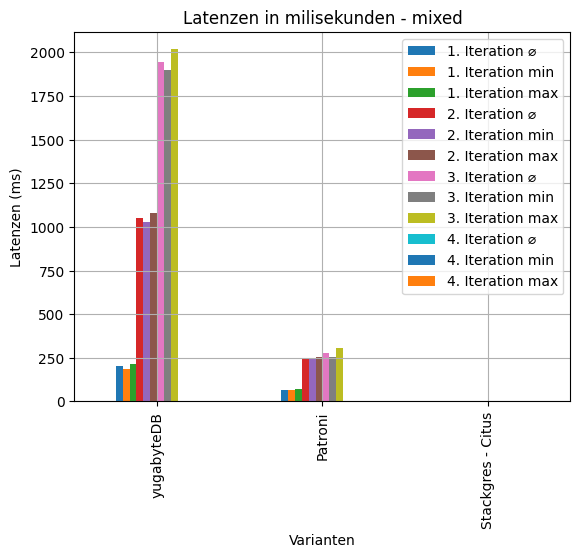
\includegraphics[width=1\linewidth]{source/pandas_data_chart_plotter/latency_mixed}
        \caption{Benchmarks - latency mixed}
        \label{fig:latency_mixed}
    \end{figure}

    \begin{figure}[H]
        \centering
        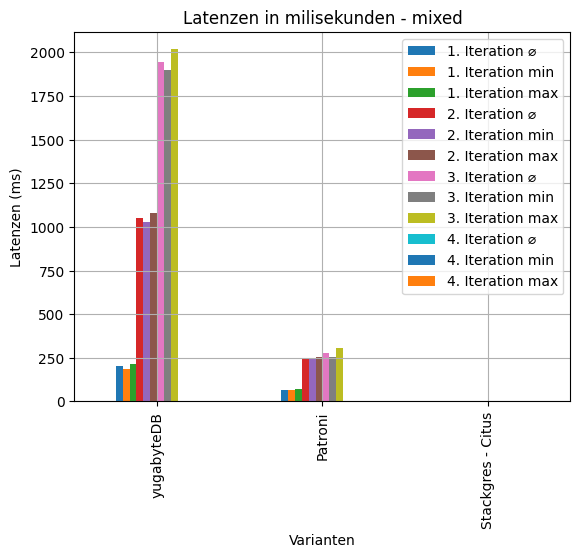
\includegraphics[width=1\linewidth]{source/pandas_data_chart_plotter/latency_dql}
        \caption{Benchmarks - latency dql}
        \label{fig:latency_dql}
    \end{figure}
\end{flushleft}
\begin{flushleft}
    \begin{warning}
        4GiB Memory für die \texttt{tserver} waren offensichtlich zu knapp bemessen.
        Zumindest wenn die Tabelle 120'000'000 Rows hat und ein mixed Benchmark abgesetzt wird.

        Dies äusserte sich in einem Fehler (Absturz)auf zwei von drei \texttt{tserver}-Nodes sowie einer hohen Anzahl an Fehlern bei den mixed-Benchmarks.
        Daher wurde das Memory auf 8GiB erhöht und die komplette Testreihe erneut gestartet.
        Zudem wurden die Anzahl Fehler ebenfalls in die Benchmark-Auswertung einbezogen.
    \end{warning}
\end{flushleft}
